%#!platex ./report.tex

 \section{CaT$B%A%c%M%k$rMQ$$$?>l9g$N7k2L(B}
   $B?^(B\ref{ca_result1}, $B?^(B\ref{ca_result2}$B$K(BCaT$B%A%c%M%k$rF3F~$7$?:]$N7k2L$r<($9(B.
   $BK^Nc$d8!Dj<jK!$H$=$N7k2L$N<($7J}$O?^(B\ref{Ka_Result1}$B$HF1MM$G$"$k(B.

     \begin{figure}[H]
       \begin{subfigure}{0.5\columnwidth}
         \centering
         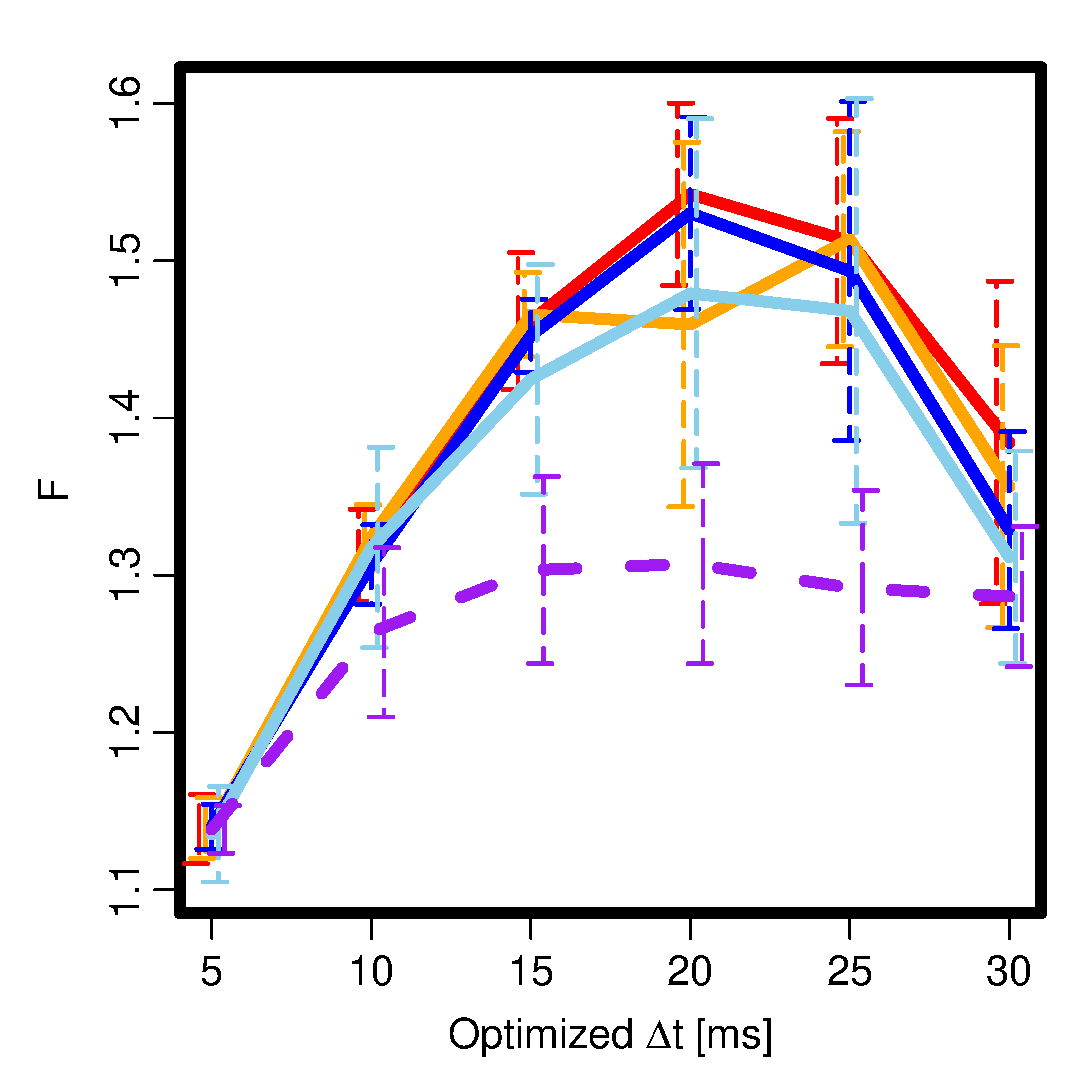
\includegraphics[width=0.8\columnwidth]{./Images_Result/ca_st50_test_F.eps}
         \caption{$F$}
         \label{ca_F}
       \end{subfigure}
       \begin{subfigure}{0.5\columnwidth}
         \centering
         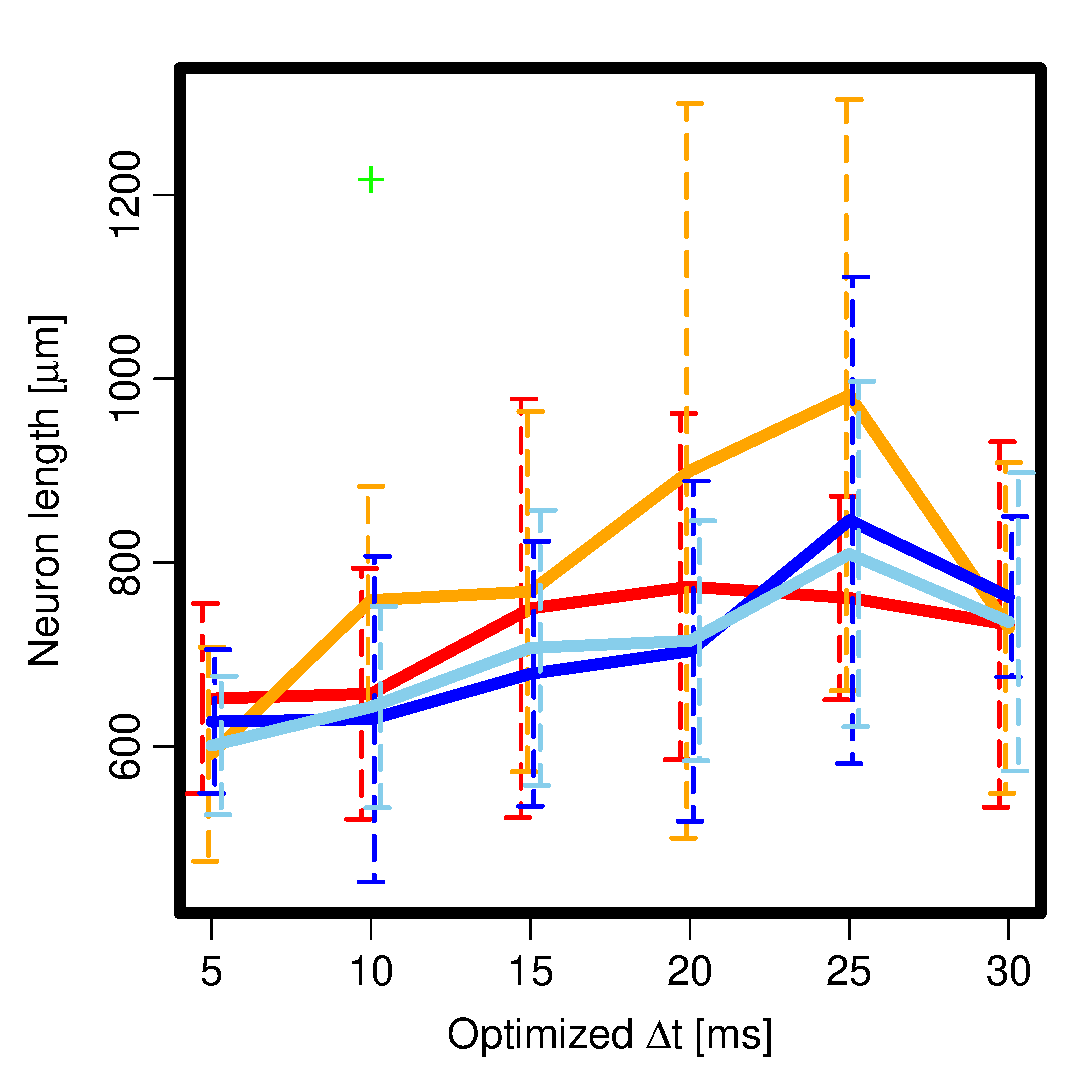
\includegraphics[width=0.8\columnwidth]{./Images_Result/ca_st50_test_TREE_length.eps} 
         \caption{$BD9$5(B}
         \label{ca_TREE_length}
       \end{subfigure}

       \begin{subfigure}{0.5\columnwidth}
         \centering
         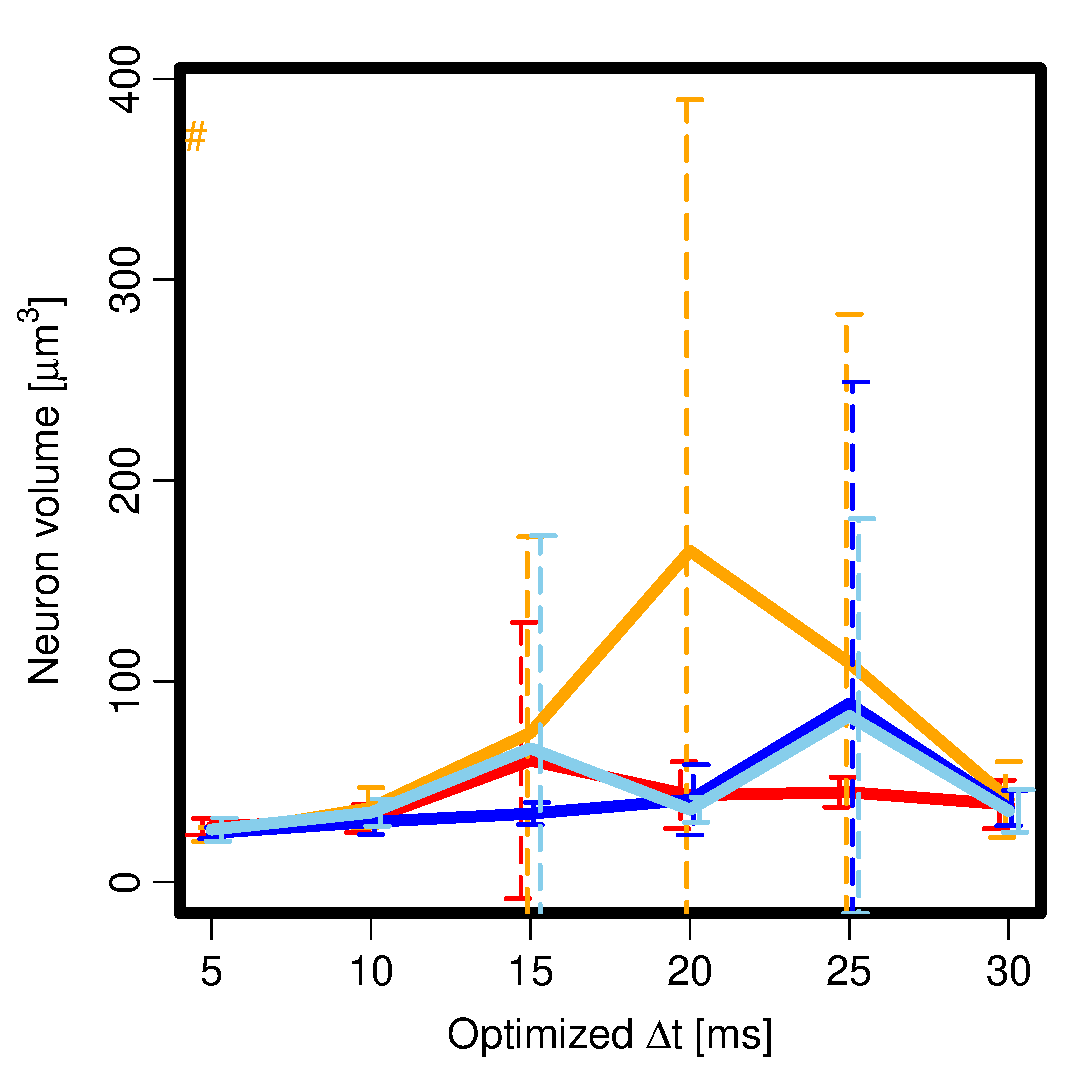
\includegraphics[width=0.8\columnwidth]{./Images_Result/ca_st50_test_TREE_volume.eps}
         \caption{$BBN@Q(B}
         \label{ca_TREE_volume}
       \end{subfigure}
       \begin{subfigure}{0.5\columnwidth}
         \centering
         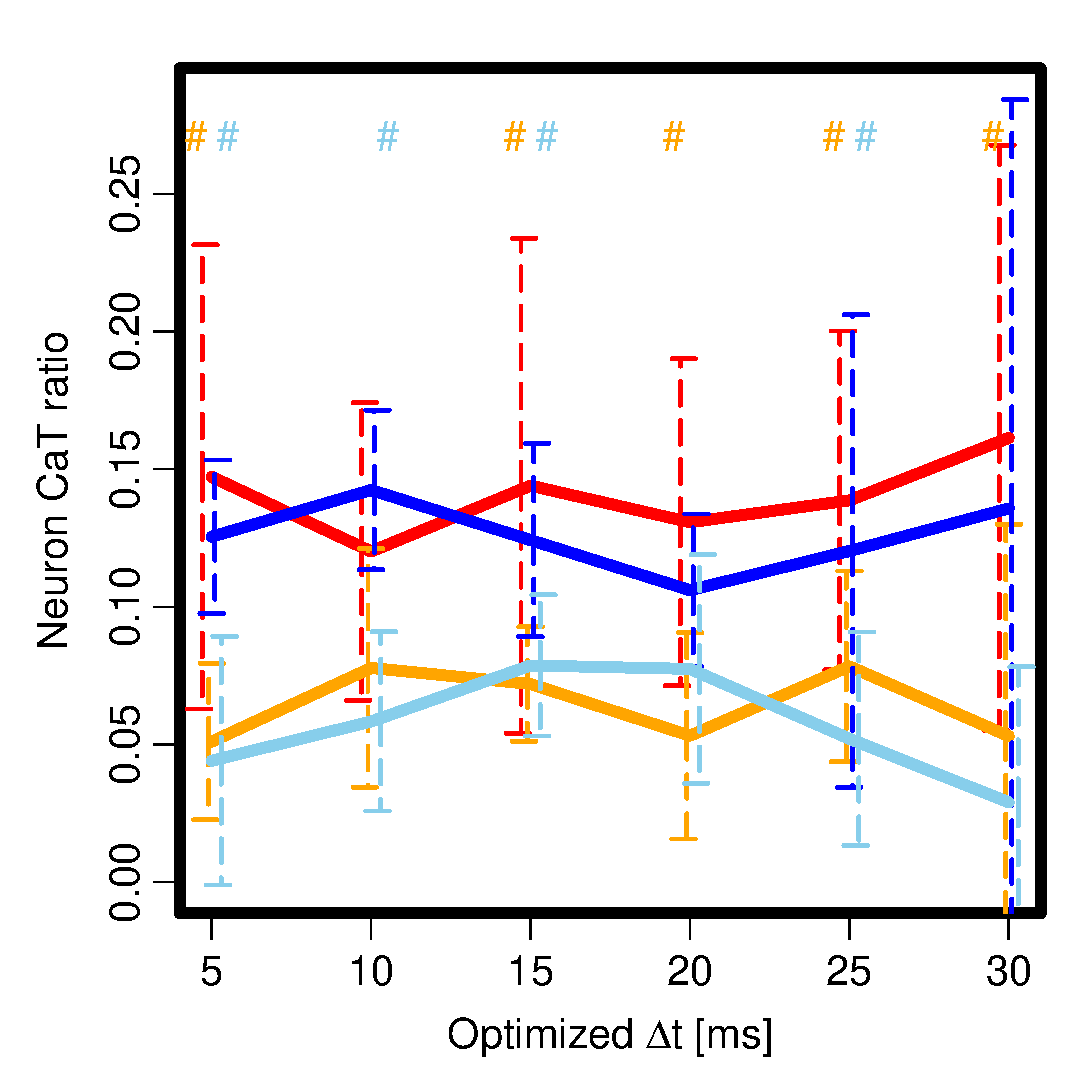
\includegraphics[width=0.8\columnwidth]{./Images_Result/ca_st50_test_TREE_Ca_ratio.eps}
         \caption{CaT$B%3%s%@%/%?%s%94^M-N((B}
         \label{ca_TREE_Ca_ratio}
       \end{subfigure}

       \vspace{-0.3cm}
       \begin{subfigure}{0.5\columnwidth}
         \centering
         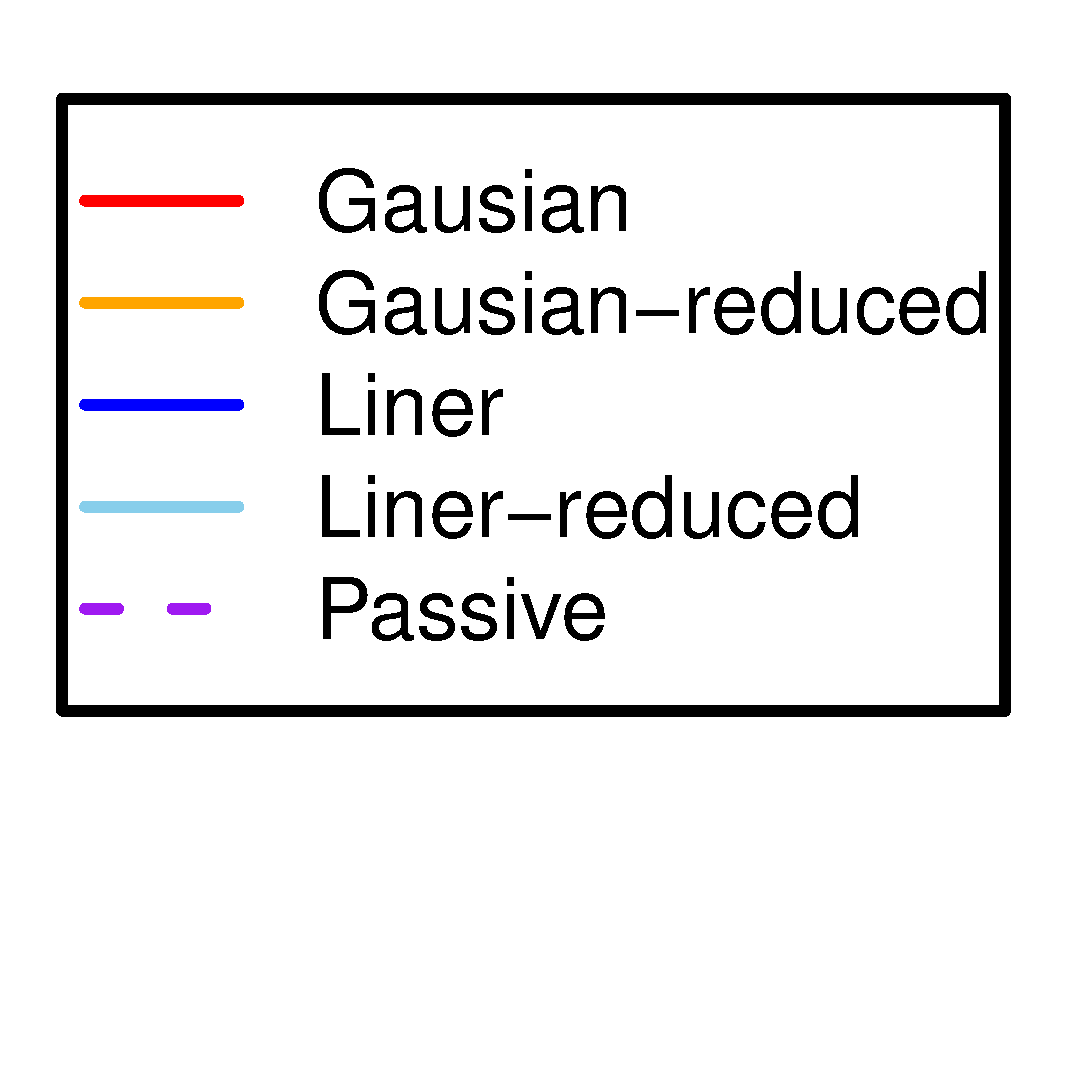
\includegraphics[width=0.6\columnwidth]{./Images_Result/ca_st50_test_legend.eps} 
       \end{subfigure}
       \begin{subfigure}{0.5\columnwidth}
         \centering
         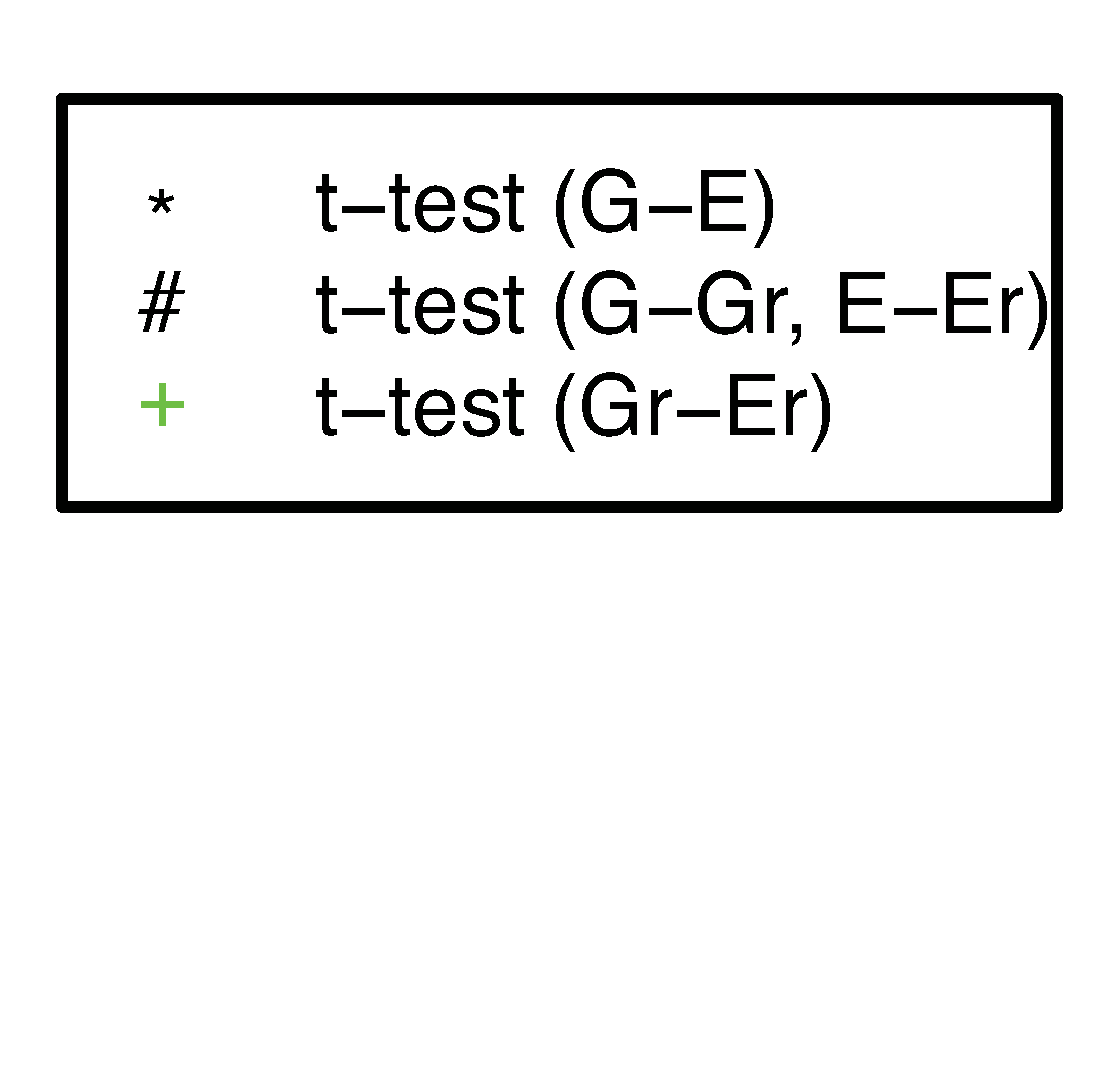
\includegraphics[width=0.6\columnwidth]{./Images_Result/exp_test_legend.eps} 
       \end{subfigure}

       \vspace{-1.6cm}
       \caption{CaT$B%A%c%M%k$rF3F~$7$?:]$N7k2L(B1} %$B%Z!<%8%l%$%"%&%H$,7hDj$7$F$+$iHyD4@0$9$k(B
       \label{ca_result1}
     \end{figure}
     $B?^(B\ref{ca_F}$B$h$j(B, CaT$B%3%s%@%/%?%s%9$rF3F~$7$?$3$H$K$h$j(BPassive$B$N>l9g$h$j$b(B
     $F$$BCM$,A}2C$7$F$$$k$3$H$,$o$+$k(B. 
     \begin{figure}[H]
       \begin{subfigure}{0.5\columnwidth}
         \centering
         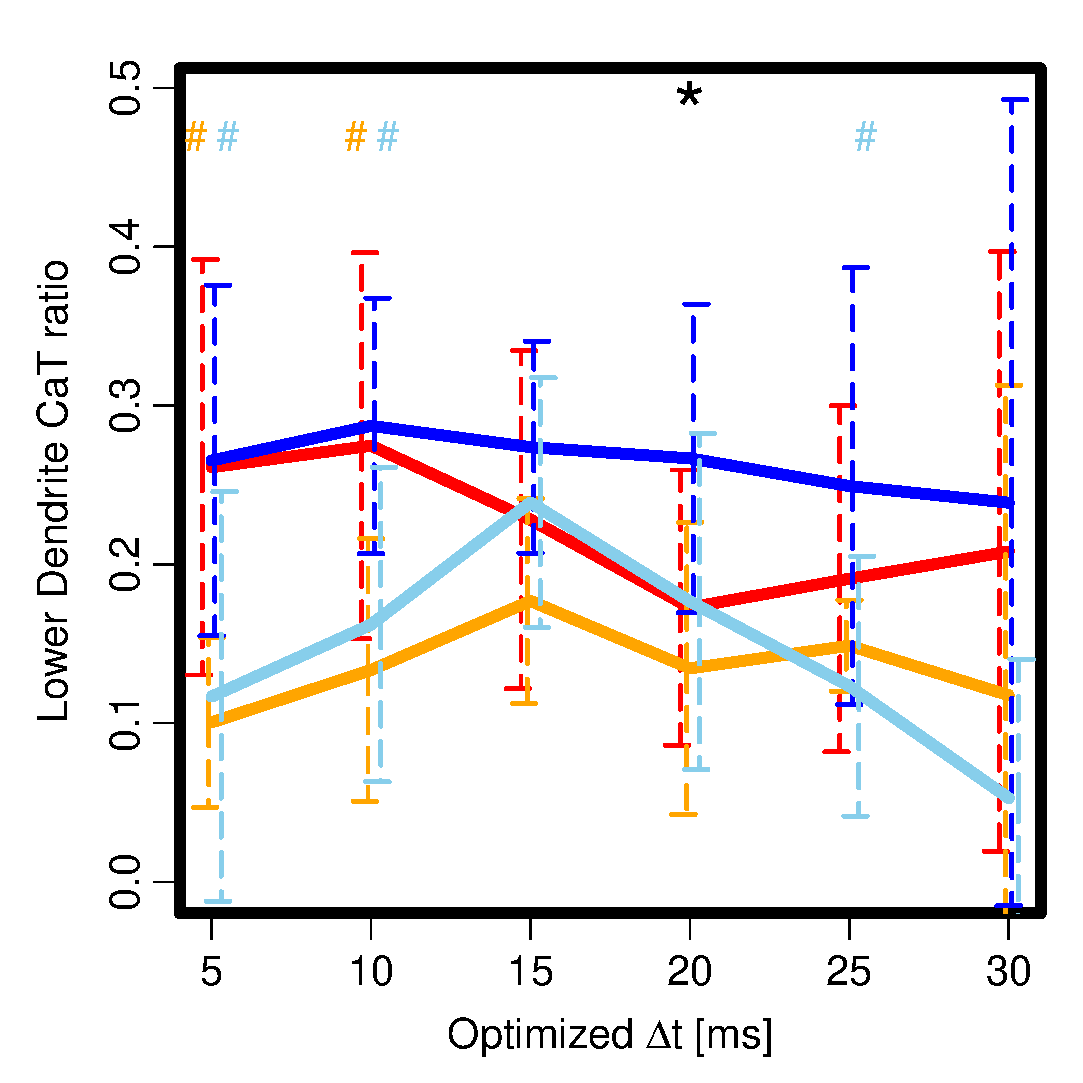
\includegraphics[width=0.8\columnwidth]{./Images_Result/ca_st50_test_Lower_Ca_ratio.eps}
         \caption{Lower Dendrite$B$N(BCaT$B%3%s%@%/%?%s%94^M-N((B}
         \label{ca_lower_ca_ratio}
       \end{subfigure}
       \begin{subfigure}{0.5\columnwidth}
         \centering
         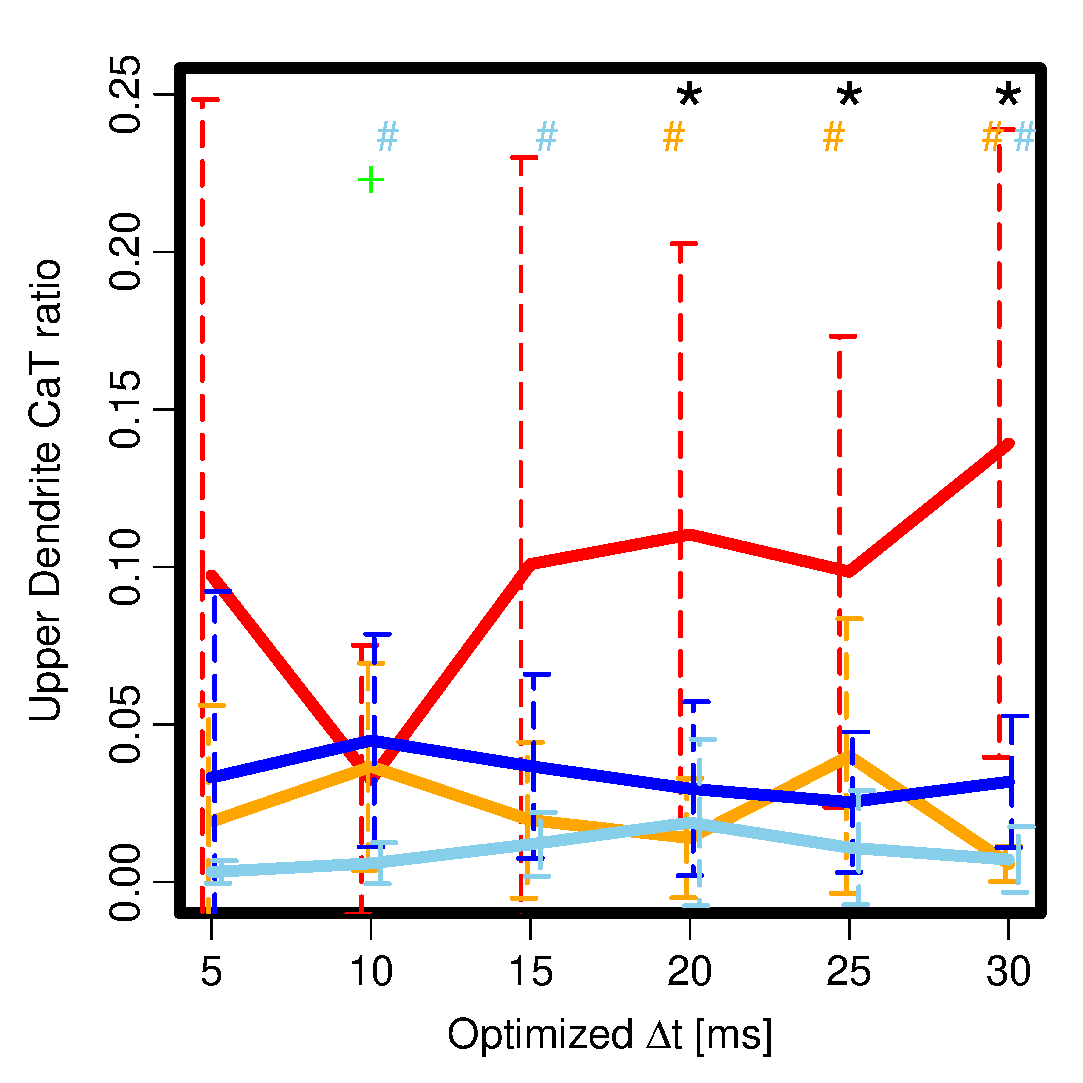
\includegraphics[width=0.8\columnwidth]{./Images_Result/ca_st50_test_Upper_Ca_ratio.eps}
         \caption{Upper Dendrite$B$N(BCaT$B%3%s%@%/%?%s%94^M-N((B}
         \label{ca_upper_ca_ratio}
       \end{subfigure}
       
       \vspace{-0.3cm}
       \begin{subfigure}{0.5\columnwidth}
         \centering
         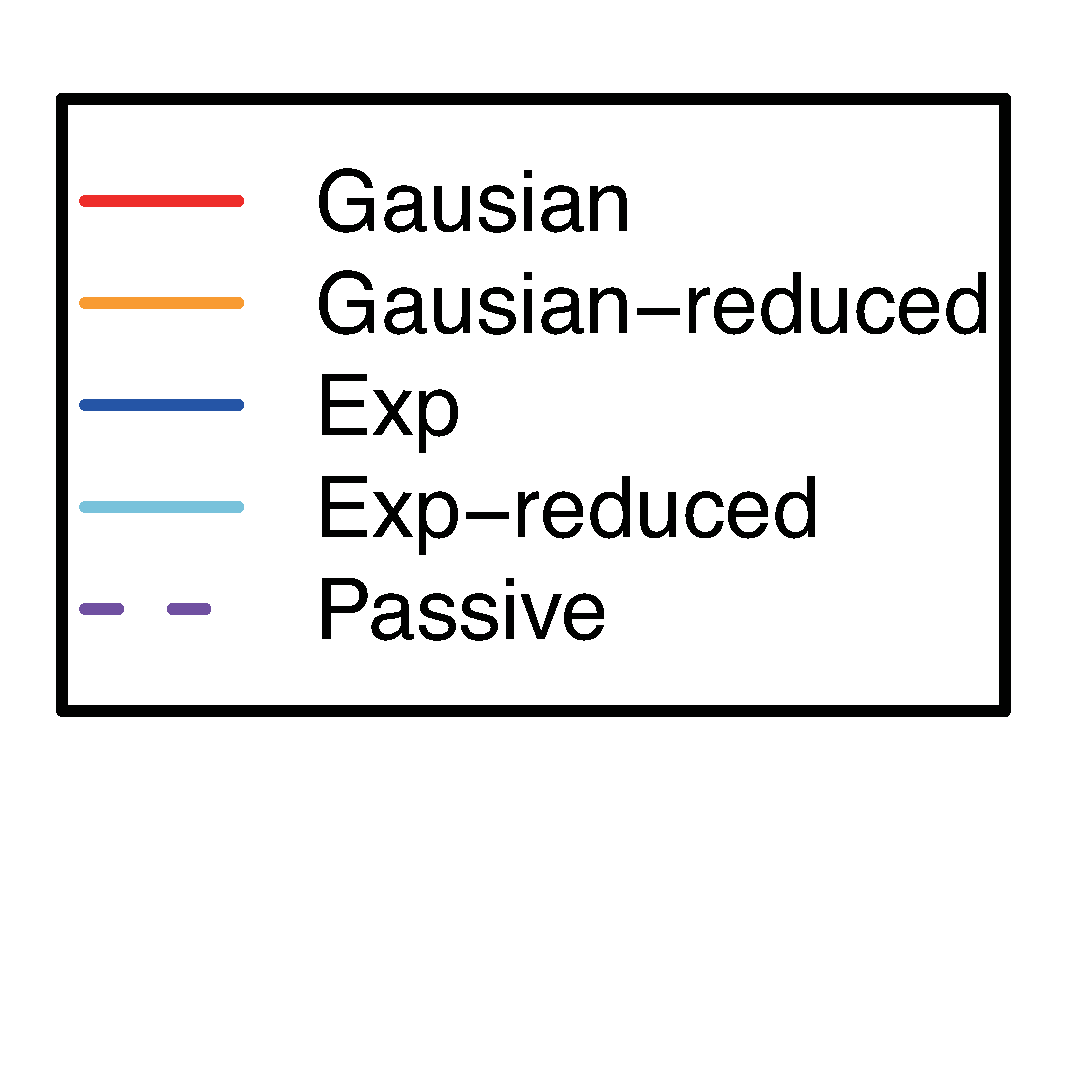
\includegraphics[width=0.6\columnwidth]{./Images_Result/exp_ca_st50_test_legend.eps} 
       \end{subfigure}
       \begin{subfigure}{0.5\columnwidth}
         \centering
         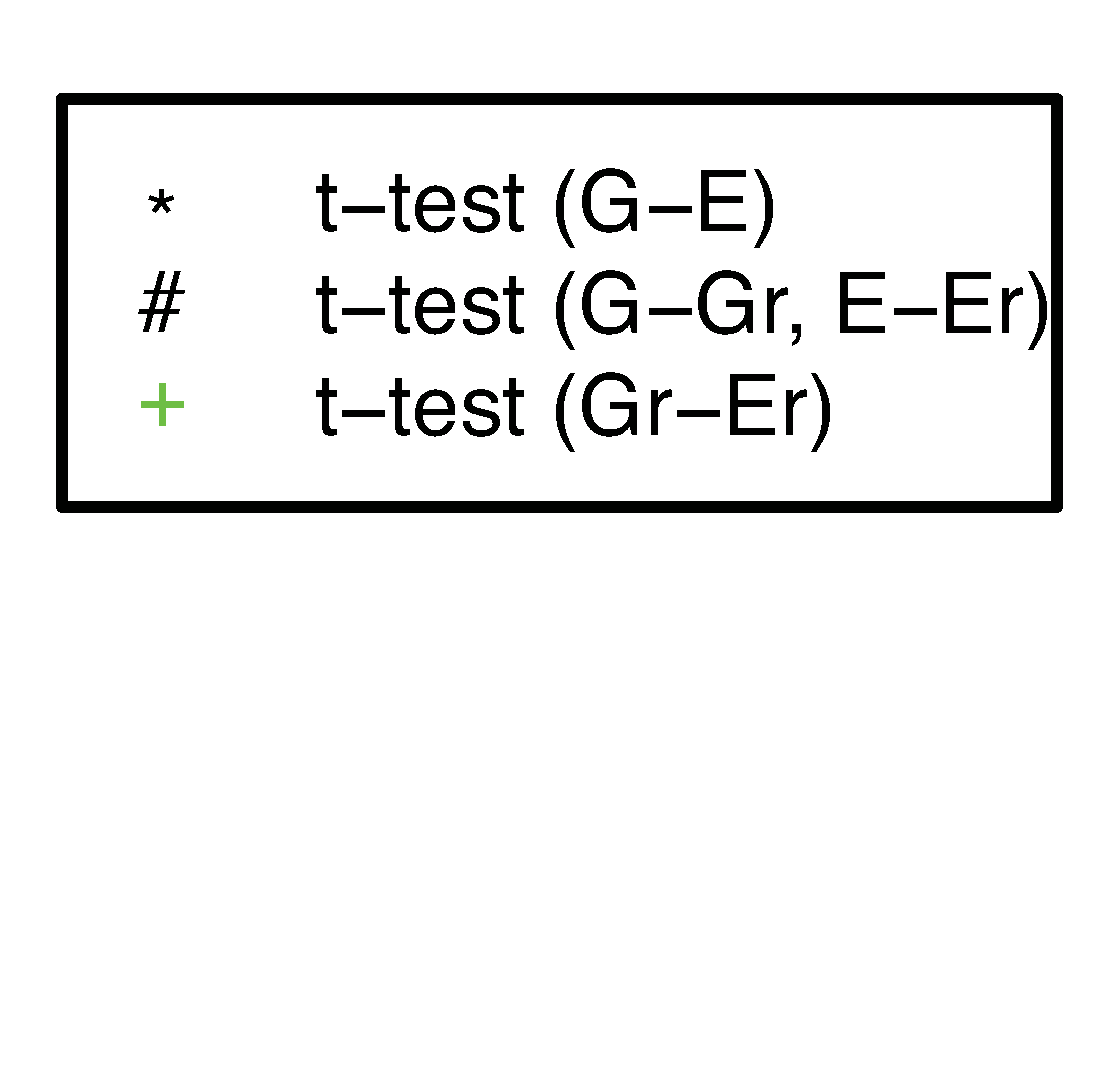
\includegraphics[width=0.6\columnwidth]{./Images_Result/exp_test_legend.eps} 
       \end{subfigure}

       \vspace{-1.6cm}
       \caption{CaT$B%A%c%M%k$rF3F~$7$?:]$N7k2L(B2} %$B%Z!<%8%l%$%"%&%H$,7hDj$7$F$+$iHyD4@0$9$k(B
       \label{ca_result2}
     \end{figure}

     $B?^(B\ref{CaT_V}$B$O(BCaT$B%3%s%@%/%?%s%9$rF3F~$7$?:]$N%7%_%e%l!<%7%g%s$N0lNc$G$"$k(B. $B<B@~$,(BCaT$B%3%s%@%/%?%s%9$rF3F~$7$?%b%G%k$NKlEE0LGH7A$G$"$j(B, 
     $BGK@~$O$=$N?@7P:YK&$+$i(BCaT$B$rIT3h@-2=(B($\overline{g}_{CaT} = 0$)$B$7$?>l9g$NKlEE0LGH7A$G$"$k(B. 
     $B?^(B\ref{CaT_V}$B$+$i$o$+$k$h$&$K(BCaT$B%3%s%@%/%?%s%9$rF3F~$9$k$H:YK&BN$G$NC&J,6K$OBg$-$/$J$j(B, $B$^$?EE0L$,9b$$>uBV$,0];}$5$l$k(B.

     \vspace{-1cm}
     \begin{figure}[H]
       \begin{subfigure}{0.5\columnwidth}
         \centering
         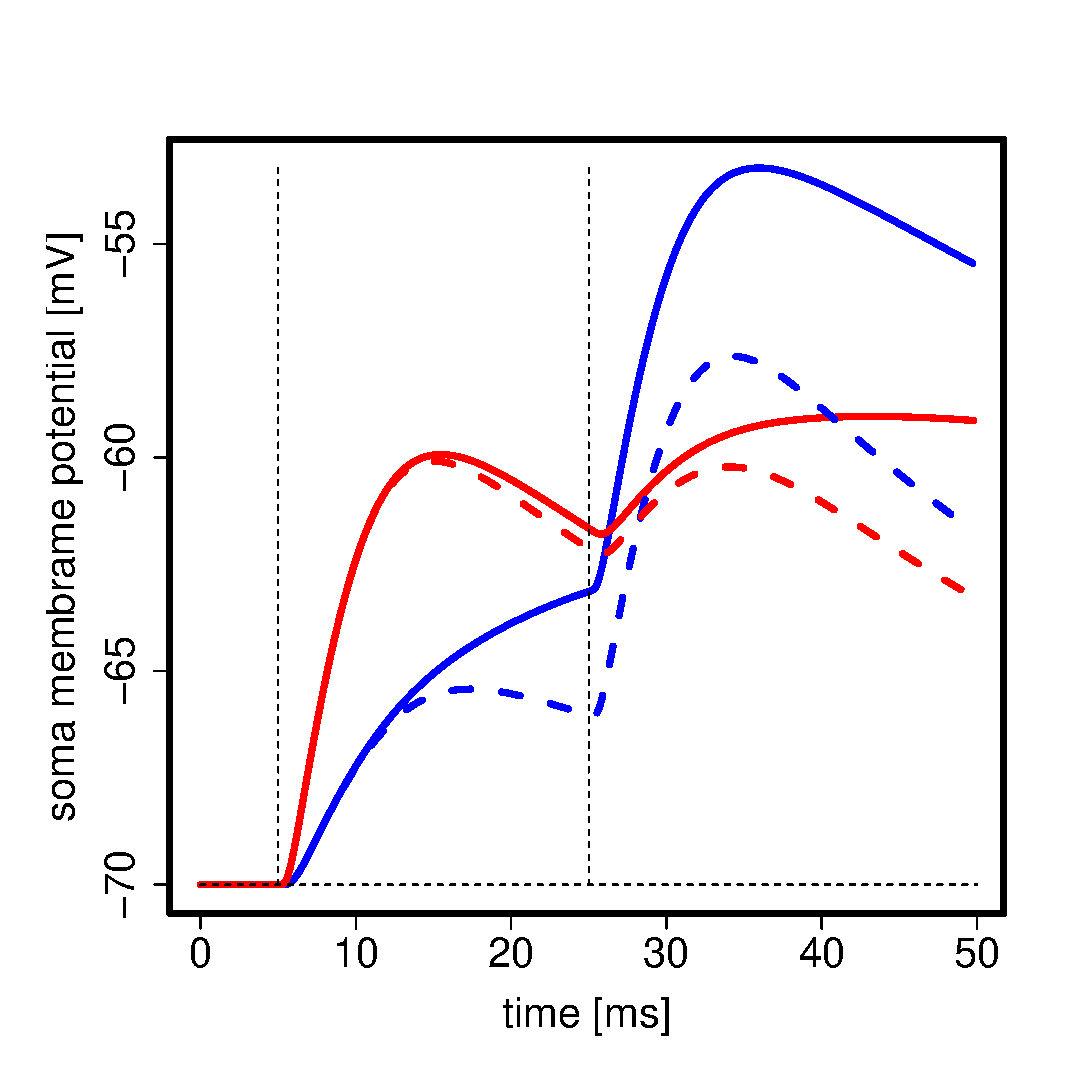
\includegraphics[width=\columnwidth]{./Images_Result/ca_st50_V_dt20_C5.eps}
       \end{subfigure}
       \begin{subfigure}{0.5\columnwidth}
         \centering
         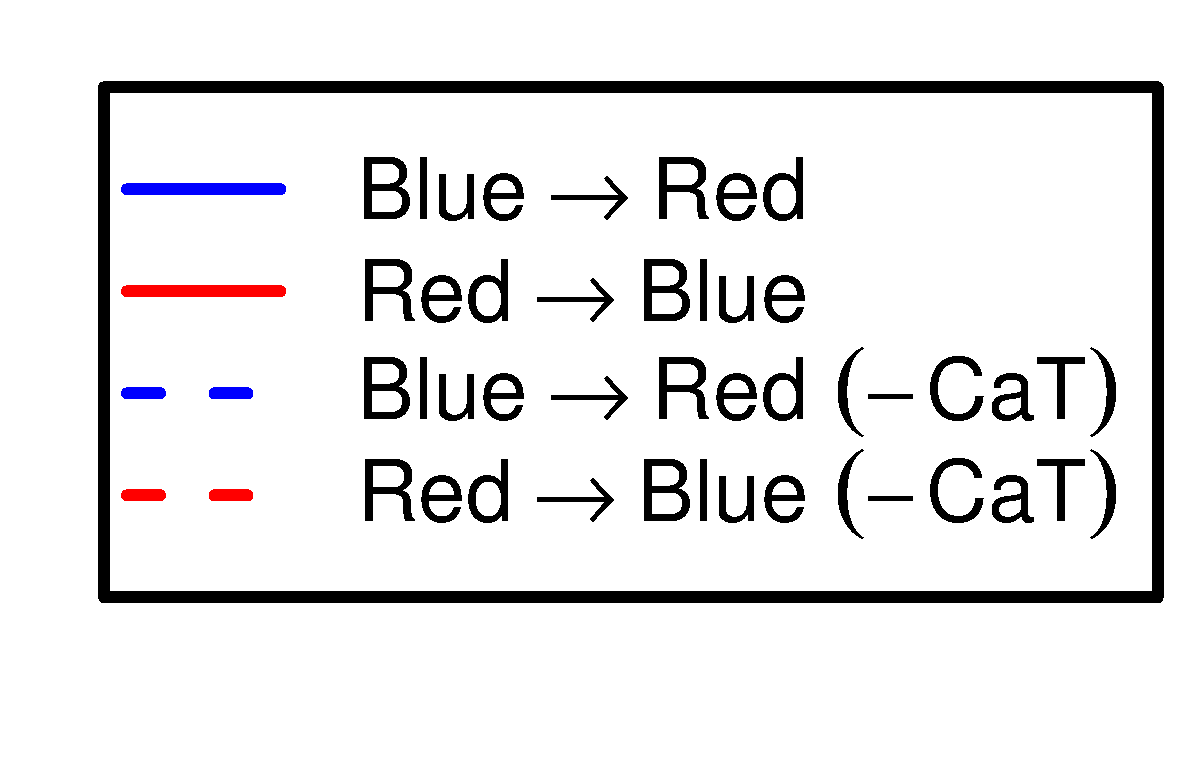
\includegraphics[width=0.8\columnwidth]{./Images_Result/ca_2simulation_legend.eps}
       \end{subfigure}
       \caption{CaT $BKlEE0LGH7ANc(B(${\Delta}t = 20$[ms])}
       \label{CaT_V}
     \end{figure}

     % $B<B:]!"8+$?L\$N7A$O$=$s$J$KBg:9$J$$$N$GE=$i$J$$$G$b$$$$$H$*$b$&(B
     
     %% $B?^(B\ref{Ca_morphos}$B$K(BCaT$B%A%c%M%k$rF3F~$7$??@7P:YK&$N7ABVNc$r<($9(B.
     %% \begin{figure}[H]
     %%   \begin{subfigure}{0.5\columnwidth}
     %%     \centering
     %%     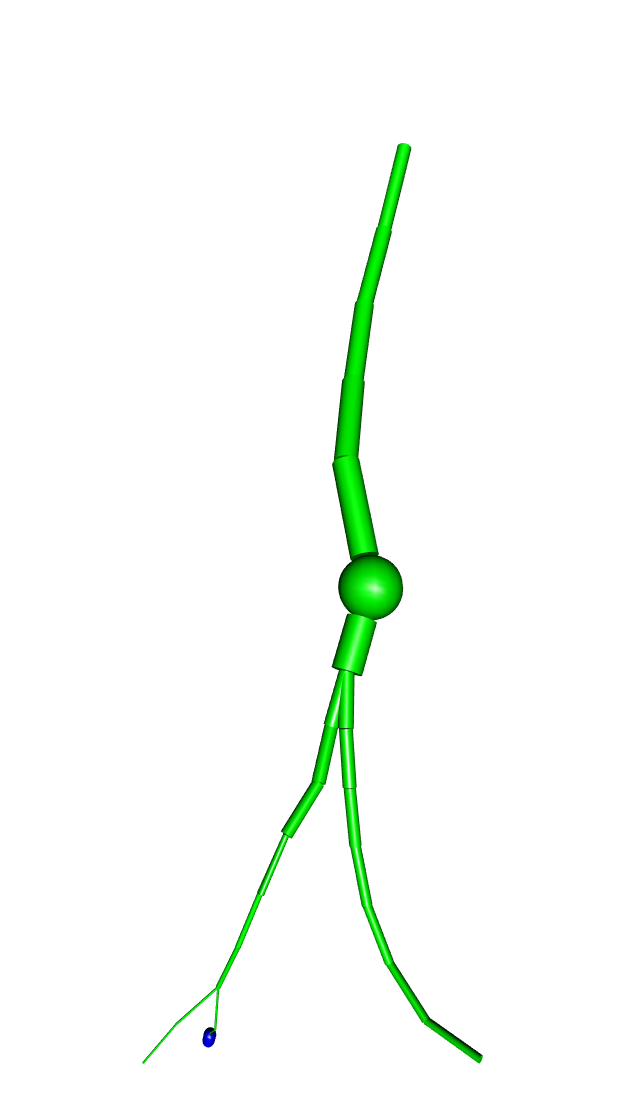
\includegraphics[width=0.5\columnwidth]{./Images_Result/alfa_sample.png} 
     %%     \caption{$B@h9T8&5f<jK!(B}
     %%  \label{Tsuishi_sampel}
     %%   \end{subfigure}
     %%   \begin{subfigure}{0.5\columnwidth}
     %%     \centering
     %%     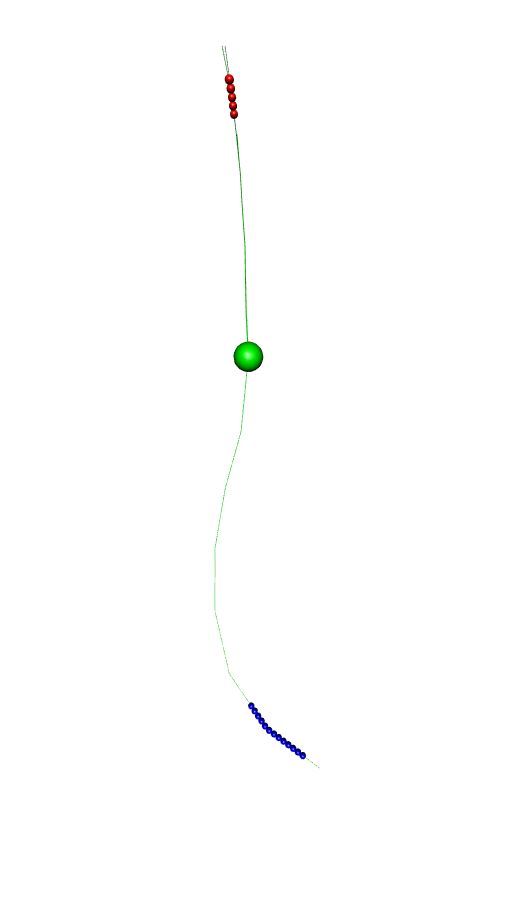
\includegraphics[width=0.3\columnwidth]{./Images_Result/rerative_sample.png}
     %%     \caption{$BK\8&5f<jK!(B}
     %%     \label{Rerative_sampel}
     %%   \end{subfigure}
     %%   \caption{CaT$B%3%s%@%/%?%s%9$rF3F~$7$??@7P:YK&$N7ABVNc(B}
     %%   \label{Ca_morphos}
     %% \end{figure}

     $B?^(B\ref{ca_Ca_dist}$B$K(B${\Delta}t = 30$[ms]$B$H$7$F:n@.$7$??@7P:YK&$N(B
     CaT$B%3%s%@%/%?%s%9J,I[$r<($9(B.
     $B?^(B\ref{ca_liner_dist}$B$H?^(B\ref{ca_liner_reduced_dist}$B$O;X?t4X?tJ,I[$rMQ$$(B,
     $B?^(B\ref{ca_gaus_dist}$B$H?^(B\ref{ca_gaus_reduced_dist}$B$O%,%&%9J,I[$rMQ$$$F$$$k(B.
     $B?^(B\ref{ca_liner_reduced_dist}$B$H?^(B\ref{ca_gaus_reduced_dist}$B$O8DBNI>2A$K(B
     $B%3%s%@%/%?%s%9$N9MN8$rF~$l$?>l9g(B(reduced)$B$G$"$k(B. 
     \vspace{-0.5cm}
     \begin{figure}[H]
       \hspace*{-2cm}
       \begin{subfigure}{0.62\columnwidth}
         \centering
         \includegraphics[width=\columnwidth]{./Images_Result/exp_ca_Rerative_liner_st50_75_0_Ca_distribution_dt20.eps}
         \caption{$B;X?t4X?tJ,I[(B}
         \label{ca_liner_dist}
       \end{subfigure}
       \begin{subfigure}{0.62\columnwidth}
         \centering
         \includegraphics[width=\columnwidth]{./Images_Result/exp_ca_Rerative_liner_st50_75_5_Ca_distribution_dt20.eps}
         \caption{$B;X?t4X?tJ,I[(B(reduced)}
         \label{ca_liner_reduced_dist}
       \end{subfigure}

       \vspace{-1.5cm}
     \begin{subfigure}{\columnwidth}
       \centering
       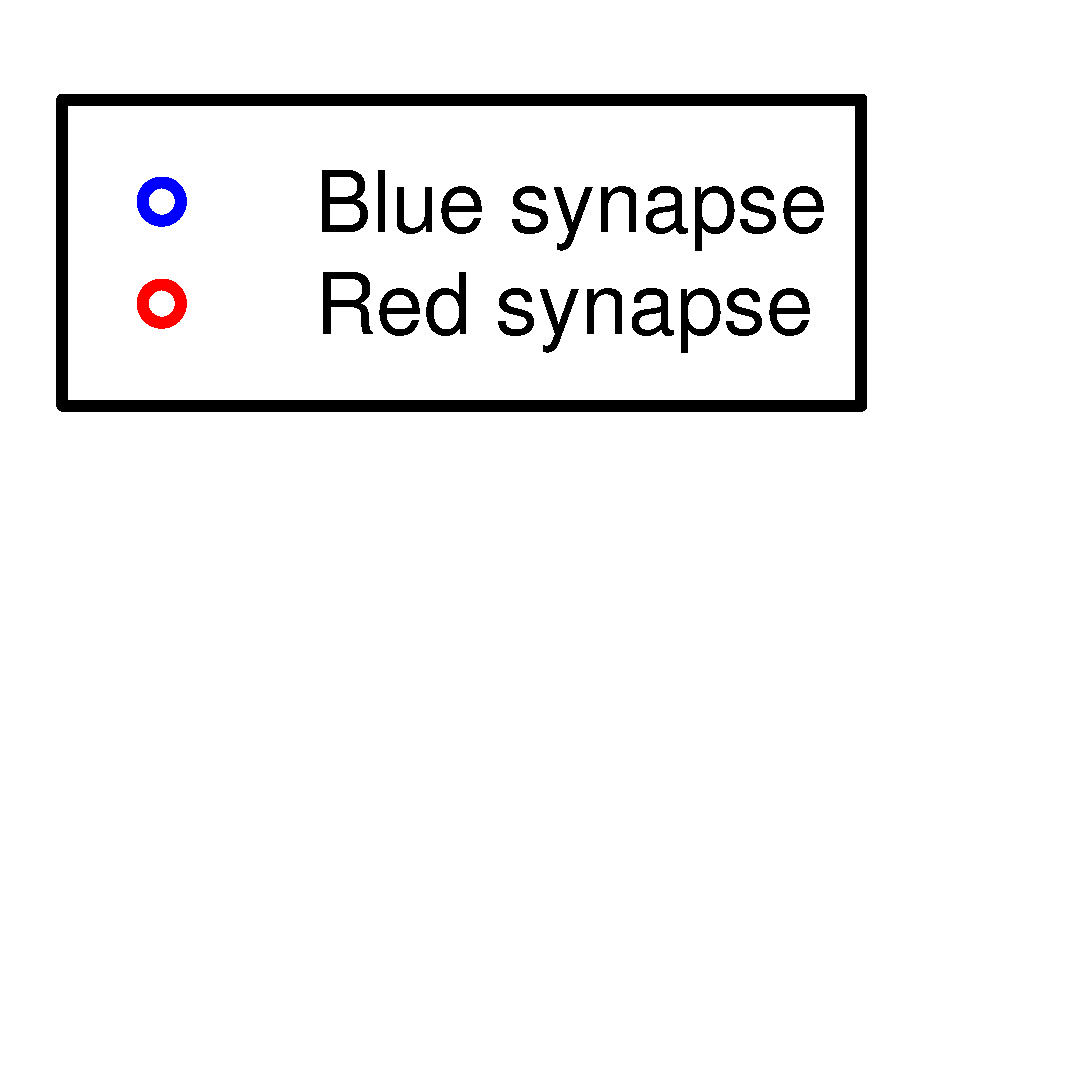
\includegraphics[width=0.35\columnwidth]{./Images_Result/Synapse_legend.eps} 
     \end{subfigure}
     \vspace{-4cm}

       \hspace*{-2cm}
       \begin{subfigure}{0.62\columnwidth}
         \centering
         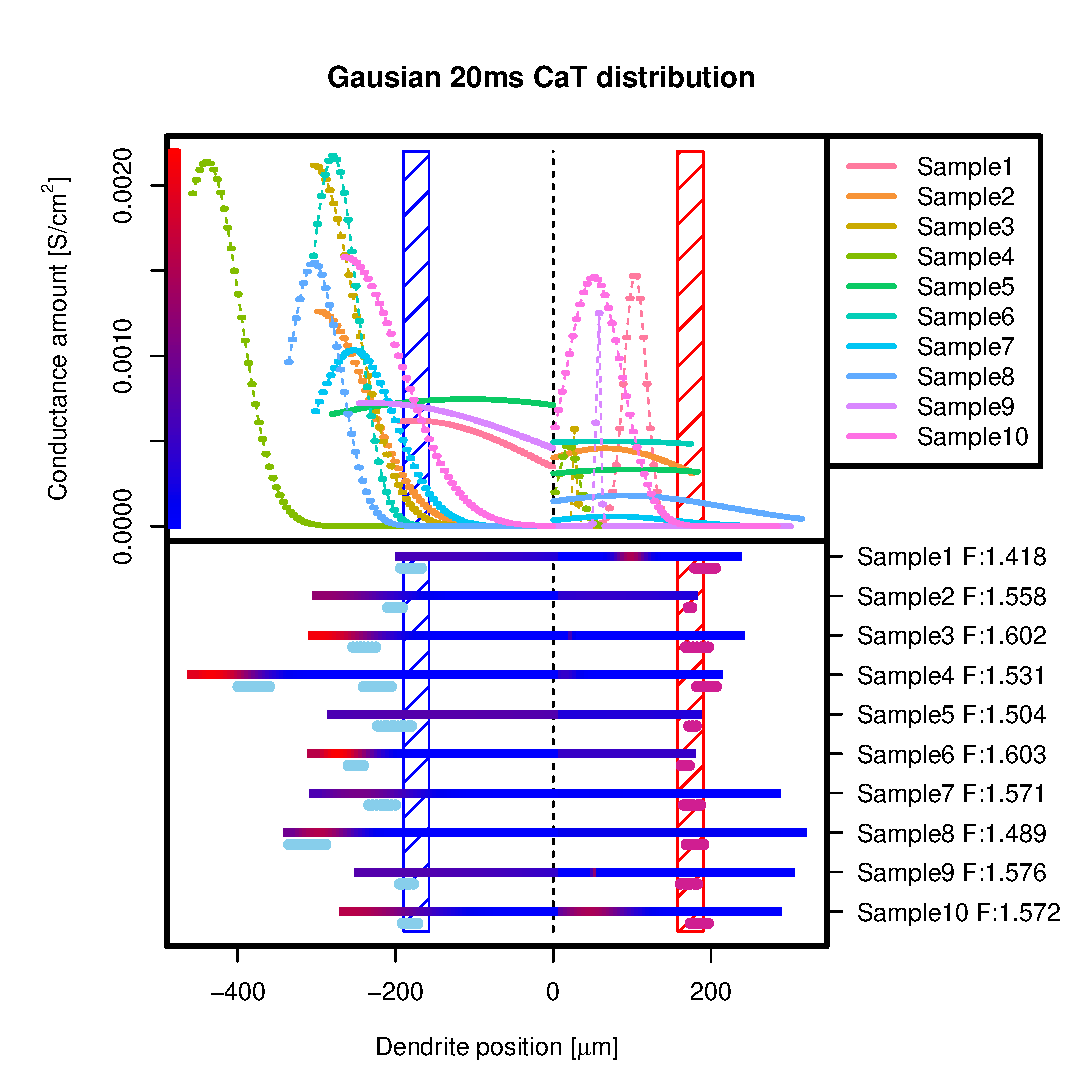
\includegraphics[width=\columnwidth]{./Images_Result/ca_Rerative_Gaus_st50_75_0_Ca_distribution_dt20.eps}
         \caption{$B%,%&%9J,I[(B} %$B$3$N%,%&%9J,I[$N?^$O%7%J%W%F%#%C%/%>!<%s$r:n$jD>$7$?$[$&$,$$$$(B
         \label{ca_gaus_dist}
       \end{subfigure}
              \begin{subfigure}{0.62\columnwidth}
         \centering
         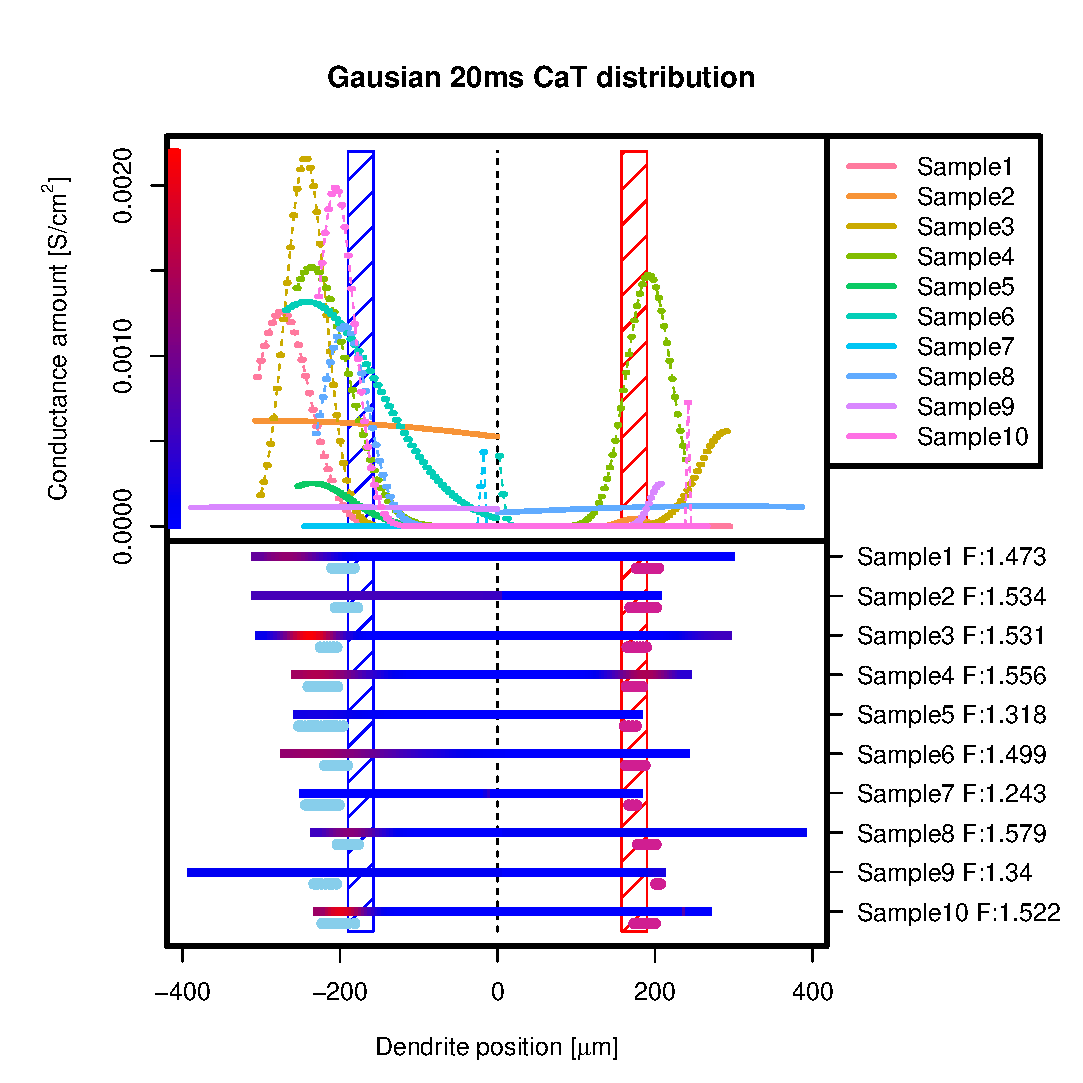
\includegraphics[width=\columnwidth]{./Images_Result/ca_Rerative_Gaus_st50_75_5_Ca_distribution_dt20.eps}
         \caption{$B%,%&%9J,I[(B(reduced)} %$B$3$N%,%&%9J,I[$N?^$O%7%J%W%F%#%C%/%>!<%s$r:n$jD>$7$?$[$&$,$$$$(B
         \label{ca_gaus_reduced_dist}
       \end{subfigure}

       \caption{${\Delta}t = 20$[ms], $B$G$N(BCaT$B%3%s%@%/%?%s%9J,I[(B}
       \label{ca_Ca_dist}
     \end{figure}

     $B?^(B\ref{ca_Ca_dist}$B$h$j(B, $B%3%s%@%/%?%s%9J,I[MM<0$K8B$i$:(BCaT$B%3%s%@%/%?%s%9$O(BLower Dendrite$B$N(B
     $B@hC<$KB?$/J,I[$7$F$$$k$3$H$,$o$+$k(B. $B8DBNI>2A$K$F%3%s%@%/%?%s%9NL$rI>2A$7$J$$>l9g$O(BUpper
     Dendrite$B$G$b(BCaT$B%3%s%@%/%?%s%9$NJ,I[$,8+$i$l$k$,(B, $BI>2A$K%3%s%@%/%?%s%9$N9MN8$rF3F~$9$k$H(B
     $B$[$H$s$I8+$i$l$J$/$J$C$?(B.
